\pdfoutput=1
\documentclass[11pt,a4paper]{article}

% ---------------------------------------------------------------------------
% A critical-point criterion for D-stability in every dimension.
% Author metadata: set the macros below before submission.
% ---------------------------------------------------------------------------
\newcommand{\PaperAuthor}{}
\newcommand{\PaperAffiliation}{}
\newcommand{\PaperDate}{September 2026}

\usepackage[T1]{fontenc}
\usepackage[utf8]{inputenc}
\usepackage{lmodern}
\usepackage[expansion=false]{microtype}
\usepackage[a4paper,margin=1.05in]{geometry}
\usepackage{amsmath,amssymb,amsthm,mathtools}
\usepackage{booktabs}
\usepackage{array}
\usepackage{enumitem}
\usepackage{graphicx}
\usepackage{caption}
\captionsetup[table]{justification=raggedright,singlelinecheck=false}
\usepackage{xcolor}
\usepackage[hyphens]{url}
\usepackage[colorlinks=true,linkcolor=blue!55!black,citecolor=blue!55!black,urlcolor=blue!55!black]{hyperref}
\hypersetup{pdftitle={A critical-point criterion for D-stability in every dimension},
  pdfauthor={\PaperAuthor},
  pdfsubject={D-stability, critical point method, time-scale robustness},
  pdfkeywords={D-stability, diagonal scaling, critical point method, Fritz John conditions, Lotka-Volterra, decentralized integral control, Lean 4}}

\setlist{itemsep=2pt,topsep=3pt}
\setlength{\emergencystretch}{2em}
\renewcommand{\UrlBreaks}{\do\_\do\.\do\/}
\newcommand{\lean}[1]{\path{#1}}
\newcolumntype{L}[1]{>{\raggedright\arraybackslash}p{#1}}

\theoremstyle{plain}
\newtheorem{theorem}{Theorem}[section]
\newtheorem{proposition}[theorem]{Proposition}
\newtheorem{lemma}[theorem]{Lemma}
\newtheorem{corollary}[theorem]{Corollary}
\theoremstyle{definition}
\newtheorem{definition}[theorem]{Definition}
\newtheorem{example}[theorem]{Example}
\newtheorem{remark}[theorem]{Remark}

\newcommand{\R}{\mathbb{R}}
\newcommand{\C}{\mathbb{C}}
\newcommand{\Rp}{\R^n_{>0}}
\newcommand{\diag}{\operatorname{diag}}
\newcommand{\spread}{\operatorname{spread}}
\newcommand{\Pre}{P_{\mathrm{re}}}
\newcommand{\Pim}{P_{\mathrm{im}}}
\newcommand{\Kk}{K_\kappa}
\newcommand{\ks}{\kappa^{*}}

% generated by make_results.py
\newcommand{\NfiveGen}{980}
\newcommand{\EpsHfloat}{0.06525}
\newcommand{\WonePattern}{$(1.96,1.96,1.11,1.00,1.00)$ for species $1,\dots,5$}
\newcommand{\CpredMinus}{3.509}
\newcommand{\CpredPlus}{8.809}
\newcommand{\CmeasMinus}{3.511}
\newcommand{\CmeasPlus}{8.815}
\newcommand{\WfourCerts}{the 60 D-stable verdicts are certified by 39 exact diagonal Lyapunov certificates and 21 rigorous exclusions, the 60 others by exact Routh counts}
\newcommand{\CheckCount}{75/75 checks passed}


\title{A critical-point criterion for D-stability in every dimension}
\author{\PaperAuthor\\[2pt]\small\PaperAffiliation}
\date{\PaperDate}

\begin{document}
\maketitle

\begin{abstract}
A real square matrix $A$ is D-stable if $DA$ is Hurwitz for every positive diagonal matrix $D$; the question
arises whenever the time scales, abundances or loop gains of the units of a linearized system are unknown.
Johnson showed that a Hurwitz matrix is D-stable iff the contact determinant $\det(iI-A\diag d)$ has no zero
with $d>0$. Applying the critical point method of real algebraic geometry to this contact set, we prove, in a
Lean~4/Mathlib formalization valid for every $n$, that $A$ is D-stable iff it is Hurwitz and an explicit
Fritz--John system in the principal minors of $-A$ has no positive solution. Criteria of this kind exist in
principle for every $n$, by quantifier elimination; ours is a specific square system with a machine-checked proof.
The system splits into a square
Lagrange system and a tangency system; for $n=5$ we state it with explicit coefficients (also in Lean). The Lean
results are equivalences; the finite decision procedure built on them rests on a generic-finiteness proposition
and a termination lemma that are proved conventionally, and it was executed exactly only for $n=3$. For $n=5$ the
Lagrange system has multihomogeneous B\'ezout number $1200$ and, numerically, $\NfiveGen$ generic complex
solutions. We prove in Lean that regular contacts persist under perturbation, so every Hurwitz boundary point of
the D-stable set is either D-stable with no contact or carries only tangential contacts, and we give an exact
example in which the Lagrange system has no solution although the matrix is not D-stable. We give an exact,
Lean-verified criterion for stability under bounded time-scale ratios, prove that near contact-free boundary
points destabilization requires unbounded time-scale separation, show that the minimal destabilizing ratio
$\ks$ is attained, and compute it with certified brackets. Worked examples: a five-species Lotka--Volterra
community, a published refinery-column gain matrix, and a family whose D-stability window is recovered
automatically.
\end{abstract}

\section{Introduction}\label{sec:intro}

A real $n\times n$ matrix $A$ is \emph{D-stable} if $DA$ is Hurwitz (all eigenvalues in the open left
half-plane) for every diagonal matrix $D$ with positive diagonal. The notion goes back to
Arrow and McManus~\cite{ArrowMcManus1958}; it is natural whenever a linear or linearized system is known up to
unknown positive rates. Table~\ref{tab:dictionary} lists three settings used below.

\begin{table}[h]
\centering\small
\caption{Where diagonal scalings come from. In each row ``$A$ is D-stable'' means stability for every choice of
the positive quantities in the third column.}\label{tab:dictionary}
\begin{tabular}{@{}L{0.2\linewidth}L{0.27\linewidth}L{0.18\linewidth}L{0.27\linewidth}@{}}
\toprule
Setting & Model & Scaling $D$ & D-stability means \\
\midrule
Lotka--Volterra communities & $\dot x_i=x_i(r_i+(Ax)_i)$ & equilibrium abundances $x^{*}$ & every feasible coexistence equilibrium is linearly stable (Jacobian $\diag(x^{*})A$; every $x^{*}>0$ is feasible for $r=-Ax^{*}$) \\
Process units & $\dot x_i=f_i(x)/V_i$ & inverse hold-ups $1/V_i$ & steady state stable for all hold-ups \\
Decentralized integral control & loops $k_i/s$ on $G(s)$ & loop gains $k_i$ & low-gain stability for all gains; see Section~\ref{sec:w2} \\
\bottomrule
\end{tabular}
\end{table}

\paragraph{Status of the problem.} D-stability of $2\times2$ matrices is equivalent to $-A$ being a
$P_0^+$-matrix~\cite{JohnsonCR1974JRNBS}. Cain~\cite{Cain1976} characterized the $3\times3$ case in closed form
with radicals. Kanovei and Logofet~\cite{KanoveiLogofet1998} gave a $4\times4$ criterion through local extrema of a
coordinate on a Hurwitz hypersurface, and Impram, Johnson and Pavani~\cite{ImpramJohnsonPavani2005} studied
robust D-stability for $n=4$. The surveys~\cite{Kushel2019,GiorgiZuccotti2015} list no complete explicit criterion for $n\ge5$;
Burlakova's conditions for $n=5$~\cite{Burlakova2009} are described in the literature as partial. Several equivalent
Johnson-type reformulations are collected in~\cite{KushelPavani2022}. D-stability is decidable for every fixed $n$
by quantifier elimination: the D-stable matrices form the complement of a semialgebraic
set~\cite{JohnsonTesi1999}. Kushel~\cite{Kushel2026} recently gave a necessary and sufficient elimination form for
every $n$ and still describes the case $n>4$ as open. A statement of the form ``$A$ is D-stable iff an explicit
polynomial system has no positive solution'' is therefore available in principle for every $n$; the criterion below
is of the same kind as the $4\times4$ criterion of Kanovei and Logofet, with a specific square system, stated
explicitly for $n=5$ and checked by machine. The interior of the D-stable set was described by Hartfiel~\cite{Hartfiel1980} and
Abed~\cite{Abed1986} (strong D-stability); see also Cross~\cite{Cross1978}. Deciding D-stability is
coNP-hard~\cite{companion_conp}. No proof in this paper depends on the companion
manuscripts~\cite{companion_attach,companion_conp}; they supply this hardness result as context and two test
families (Example~\ref{ex:bh} and the coNP gadgets of Section~\ref{sec:validation}).

\paragraph{The method is classical.} The starting point is Johnson's criterion~\cite{JohnsonCR1975JME}: a Hurwitz
matrix is D-stable iff $\det(iI-A\diag d)$ has no zero with $d>0$ (Lemma~\ref{lem:johnson}). To certify emptiness
of this real set we use the foundational lemma of the \emph{critical point method}~\cite{GrigorievVorobjov1988,Renegar1992a,Renegar1992b,Renegar1992c,BasuPollackRoy2006,AubryRouillierSafeyElDin2002,SafeyElDinSchost2003}:
a proper function attains its minimum on a nonempty closed set, and the minimizer is a Fritz--John point.
Degree bounds for critical-point systems of the multihomogeneous kind below are in~\cite{SafeyElDinSpaenlehauer2016},
and the handling of open orthants by an inequation in~\cite{BerthomieuGillotSafeyElDin2026}. Our contribution is
the application of this method to Johnson's contact set, its formal proof, and the consequences below, not the
method itself.

\paragraph{Results and their status.} We label every statement: \emph{Lean} (formalized in Lean~4 with Mathlib,
compiled with warnings treated as errors; Section~\ref{sec:lean}), \emph{exact} (exact computation, replayed by
the ancillary script), \emph{conventional} (a complete written proof, not formalized), \emph{sketch} (a proof
outline), or \emph{numerical}.
\begin{enumerate}[label=(\roman*)]
\item \emph{Criterion, every $n$ (Lean).} $A$ is D-stable iff it is Hurwitz and the Fritz--John system of a proper
exhaustion on the contact set has no positive solution (Theorem~\ref{thm:coverage}); in principal-minor
coordinates it splits into a Lagrange branch and a tangency branch (Theorem~\ref{thm:explicit},
Corollary~\ref{cor:branches}), stated with explicit coefficients for $n=5$ (Theorem~\ref{thm:five}). These are
equivalences, not decision procedures. The coverage argument removes the treatment of critical points at
infinity that the argument of~\cite{KanoveiLogofet1998} does not address explicitly for $n=4$.
\item \emph{The equality branch (Lean and conventional).} Regular contacts persist under perturbation
(Theorem~\ref{thm:robust}); hence a Hurwitz matrix in the closure of the D-stable set is either D-stable without
contact or not D-stable with only tangential contacts (Theorem~\ref{thm:dichotomy}). An exact example shows that
the tangency branch cannot be dropped (Example~\ref{ex:b3}). A finite recursion decides the tangency branch
without any finiteness assumption (Lemma~\ref{lem:termination}, conventional).
\item \emph{Size (exact and sketch).} The Lagrange system has multihomogeneous B\'ezout number $n!\binom n2$
(Proposition~\ref{prop:bezout}) and is finite and nonsingular for generic weights (Proposition~\ref{prop:fin},
sketch). The resulting finite procedure was executed exactly for $n=3$ only.
\item \emph{Time-scale robustness (Lean and conventional).} Stability for all rate vectors with pairwise ratios at
most $\kappa$ is decided by Fritz--John points on the faces of a compact box (Theorem~\ref{thm:cone}); the
minimal destabilizing ratio $\ks$ is attained (Proposition~\ref{prop:kappa}); near a Hurwitz matrix without
contacts destabilization needs ratios beyond any bound (Theorem~\ref{thm:separation}), at a rate
$\ks\asymp\delta^{-1}$ that is only sketched (Remark~\ref{rem:p1}) and observed numerically; near nondegenerate
tangential points it does not (Proposition~\ref{prop:fragile}, conventional).
\end{enumerate}

\section{Setting}\label{sec:setting}

For $d\in\R^n$ write $\diag d$ for the diagonal matrix with entries $d_i$, and $\Rp$ for the open positive
orthant. Since $A\diag d$ and $\diag(d)A$ are similar for $d>0$, D-stability can be tested with right scalings;
we do so throughout, as the formalization does. For $S\subseteq\{1,\dots,n\}$ let $m_S=\det(-A[S])$ be the
principal minor of $-A$ on $S$, with $m_\emptyset=1$, and $d^S=\prod_{l\in S}d_l$.

\begin{definition}\label{def:contact}
The \emph{contact determinant} of $A$ is $f_A(d)=\det(iI-A\diag d)$ for $d\in\R^n$, with real and imaginary
parts $\Pre,\Pim$. A \emph{contact} is a point $d\in\Rp$ with $f_A(d)=0$; the (semialgebraic) set of contacts is
the \emph{contact set} $C_A$. Its complexification is $V_A=\{d\in\C^n:\Pre(d)=\Pim(d)=0\}$, of codimension two.
\end{definition}

A contact is a positive rate vector at which $A\diag d$ has the eigenvalue $i$. If $A\diag d$ has an
eigenvalue $i\omega$ with $\omega>0$, then $d/\omega$ is a contact. Note that $|f_A(d)|^2=\det(I+(A\diag d)^2)$, the
quantity used in~\cite{Hartfiel1980,Abed1986}.

\begin{lemma}[Principal-minor expansion; Lean]\label{lem:expansion}
$f_A(d)=\sum_{S\subseteq\{1,\dots,n\}} i^{\,n-|S|}\,m_S\,d^S$. In particular $\Pre$ and $\Pim$ are multiaffine
polynomials whose coefficients are principal minors of $-A$.
\end{lemma}

\begin{proof}
The $l$-th row of $(iI-A\diag d)^{\mathsf T}$ is $d_l$ times column $l$ of $-A$ plus $i$ times the unit row
$e_l$. Expanding the determinant multilinearly in the rows gives, for each $S$, the factor $i^{n-|S|}d^S$
times the determinant of the matrix whose rows are the columns of $-A$ indexed by $S$ and unit rows
elsewhere, which equals $\det(-A[S])$ by a block-triangular expansion.
\end{proof}

\begin{lemma}[Johnson's criterion~\cite{JohnsonCR1975JME}; Lean]\label{lem:johnson}
$A$ is D-stable if and only if $A$ is Hurwitz and $C_A=\emptyset$.
\end{lemma}

\begin{proof}
A contact is an eigenvalue $i$ of $A\diag d$, so D-stable matrices have none. Conversely, let $A$ be Hurwitz
without contacts. No $A\diag d$ with $d>0$ has an eigenvalue on the imaginary axis: the eigenvalue $0$ is
excluded because $A$ is nonsingular, and $i\omega$ with $\omega\neq0$ would give the contact $d/|\omega|$
(use the complex conjugate if $\omega<0$). The orthant is connected, the Hurwitz matrices and the matrices
with an eigenvalue of positive real part are open, and $A\diag\mathbf 1=A$ is Hurwitz; hence every
$A\diag d$ is Hurwitz.
\end{proof}

\section{Coverage and the explicit criterion}\label{sec:coverage}

\begin{definition}\label{def:exhaustion}
A \emph{proper exhaustion} of $\Rp$ is a function $\psi\colon\Rp\to\R$ of class $C^1$ each of whose sublevel sets
$\{d\in\Rp:\psi(d)\le r\}$ is contained in a compact subset of $\Rp$. A \emph{Fritz--John point} of $\psi$ on $C_A$ is a contact $d$
for which there is $(\Lambda_1,\Lambda_2,\Lambda_0)\neq0$ with
$\Lambda_1\nabla\Pre(d)+\Lambda_2\nabla\Pim(d)+\Lambda_0\nabla\psi(d)=0$.
\end{definition}

The weighted log barrier $\psi_{a,b}(d)=\sum_i(a_id_i-b_i\log d_i)$ with $a,b>0$ is a proper exhaustion, and
so is $\sum_i(a_id_i+b_i/d_i)$.

\begin{theorem}[Coverage; Lean]\label{thm:coverage}
Let $\psi$ be a proper exhaustion of $\Rp$. A real square matrix $A$ is D-stable if and only if $A$ is
Hurwitz and $\psi$ has no Fritz--John point on $C_A$.
\end{theorem}

\begin{proof}
If $A$ is D-stable it is Hurwitz and $C_A=\emptyset$ (Lemma~\ref{lem:johnson}), so there is no Fritz--John
point. Conversely let $A$ be Hurwitz and not D-stable. By Lemma~\ref{lem:johnson} there is a contact $d_0$.
The set $K=\{\psi\le\psi(d_0)\}\cap C_A$ is compact (a closed subset of a compact sublevel set) and contains
$d_0$, so $\psi|_K$ attains its minimum at some $d^{*}$. Contacts outside $K$ have $\psi>\psi(d_0)\ge\psi(d^{*})$,
and $\Rp$ is open, so $d^{*}$ is a local minimum of $\psi$ on $\{\Pre=0,\ \Pim=0\}$. The Lagrange multiplier rule
in Fritz--John form (no constraint qualification) gives $(\Lambda_1,\Lambda_2,\Lambda_0)\neq0$.
\end{proof}

\begin{figure}[t]
\centering
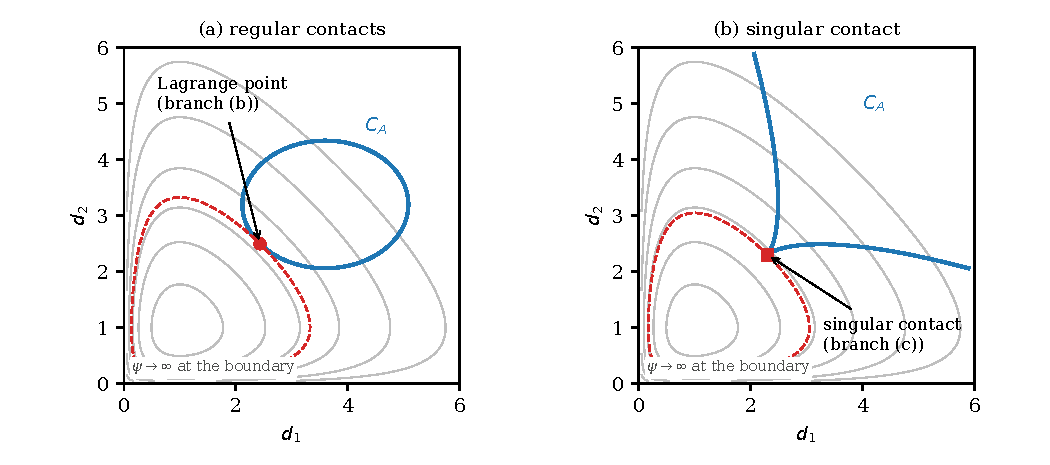
\includegraphics[width=0.92\linewidth]{figures/fig_schematic.pdf}
\caption{Schematic of the coverage argument, drawn in two dimensions (the contact set itself has dimension
$n-2$). Grey: level sets of $\psi(d)=\sum_i(d_i-\log d_i)$, which blow up at the boundary of the orthant. Blue:
contacts. The minimizer of $\psi$ over the contacts is either a regular point where a level set touches $C_A$ (a
solution of (b), panel (a)) or a singular point of $C_A$ (a solution of (c), panel (b)).}\label{fig:schematic}
\end{figure}

\begin{remark}[Relation to the $4\times4$ criterion of Kanovei and Logofet]\label{rem:kl}
Kanovei and Logofet~\cite[Thm.~5]{KanoveiLogofet1998} reduce the $4\times4$ case to a slice condition at
$z=1$ and the absence of positive local extrema of the coordinate $z$ on $T=\{f=0\}\subset\R^3_{>0}$, where $f$ is
the Hurwitz determinant of $\diag(1,x,y,z)A$; besides contacts, $T$ contains points where the scaled matrix has a
pair of real eigenvalues $\pm r$. Their argument distinguishes whether $T$ is bounded away from $z=0$ and $z=\infty$.
Two points are not addressed explicitly there: $z$ is not proper on $T$, which is closed only in the open
orthant, so extremizing sequences may escape to the boundary in $x$ or $y$ while $z$ stays bounded; and the
dichotomy uses connectedness of $z(T)$. We do not claim a counterexample to their criterion. With a proper
exhaustion neither point arises, and Theorem~\ref{thm:coverage} with $n=4$ is a complete criterion.
\end{remark}

In principal-minor coordinates the Fritz--John condition is explicit. Write
$\partial_i f_A(d)=\sum_{S\ni i}i^{\,n-|S|}m_S\,d^{S\setminus\{i\}}$.

\begin{theorem}[Explicit criterion; Lean]\label{thm:explicit}
Let $a,b\in\Rp$. $A$ is D-stable if and only if $A$ is Hurwitz and there is no $d\in\Rp$ with $f_A(d)=0$
for which some $(\Lambda_1,\Lambda_2,\Lambda_0)\neq0$ satisfies, for every $i$,
\[
\Lambda_1\,\mathrm{Re}\,\partial_if_A(d)+\Lambda_2\,\mathrm{Im}\,\partial_if_A(d)+\Lambda_0\Bigl(a_i-\frac{b_i}{d_i}\Bigr)=0 .
\]
\end{theorem}

\begin{proof}
Theorem~\ref{thm:coverage} for $\psi_{a,b}$, with the partial derivatives of Lemma~\ref{lem:expansion} evaluated
on the unit vectors.
\end{proof}

\begin{corollary}[Two branches; Lean]\label{cor:branches}
$A$ is D-stable if and only if $A$ is Hurwitz and neither of the following systems has a solution with
$d\in\Rp$:
\begin{enumerate}[label=(\alph*),start=2]
\item (Lagrange branch) $f_A(d)=0$ and, for some $\lambda,\mu\in\R$ and all $i$,
$a_id_i-b_i=\lambda\,d_i\,\mathrm{Re}\,\partial_if_A(d)+\mu\,d_i\,\mathrm{Im}\,\partial_if_A(d)$;
\item (tangency branch) $f_A(d)=0$ and, for some $t\in\R$ and all $i$,
$(1-t^2)\,\mathrm{Re}\,\partial_if_A(d)+2t\,\mathrm{Im}\,\partial_if_A(d)=0$.
\end{enumerate}
\end{corollary}

\begin{proof}
If $\Lambda_0\neq0$, divide by $\Lambda_0$ and multiply the $i$-th equation by $d_i$: this is (b) with
$\lambda=-\Lambda_1/\Lambda_0$, $\mu=-\Lambda_2/\Lambda_0$. If $\Lambda_0=0$ then $(\Lambda_1,\Lambda_2)\neq0$, and
every nonzero direction in $\R^2$ is, up to a nonzero factor, $(1-t^2,2t)$ for a real $t$: with
$r=(\Lambda_1^2+\Lambda_2^2)^{1/2}$ take $t=0$ if $\Lambda_2=0$ and $t=(r-\Lambda_1)/\Lambda_2$ otherwise.
Conversely (b) gives $(\Lambda_1,\Lambda_2,\Lambda_0)=(-\lambda,-\mu,1)$ and (c) gives $(1-t^2,2t,0)\neq0$.
\end{proof}

For $n=5$ set $c_k(d)=\sum_{|S|=k}m_Sd^S$ ($c_0=1$) and
$c_k^{(i)}(d)=\sum_{|S|=k,\,S\ni i}m_S\,d^{S\setminus\{i\}}$. Since $i^{5-k}=i,1,-i,-1,i,1$ for $k=0,\dots,5$,
Lemma~\ref{lem:expansion} gives $\Pre=c_1-c_3+c_5$ and $\Pim=1-c_2+c_4$.

\begin{theorem}[The $5\times5$ criterion; Lean]\label{thm:five}
Let $A$ be a real $5\times5$ matrix and $a,b\in\R^5_{>0}$. Then $A$ is D-stable if and only if
\begin{enumerate}[label=(\alph*)]
\item $A$ is Hurwitz;
\item there are no $d\in\R^5_{>0}$ and $\lambda,\mu\in\R$ with $c_1-c_3+c_5=0$, $1-c_2+c_4=0$ and
\[a_id_i-b_i=\lambda\,d_i\bigl(c^{(i)}_1-c^{(i)}_3+c^{(i)}_5\bigr)+\mu\,d_i\bigl(c^{(i)}_4-c^{(i)}_2\bigr)\quad(i=1,\dots,5);\]
\item there are no $d\in\R^5_{>0}$ and $t\in\R$ with $c_1-c_3+c_5=0$, $1-c_2+c_4=0$ and
\[(1-t^2)\bigl(c^{(i)}_1-c^{(i)}_3+c^{(i)}_5\bigr)+2t\bigl(c^{(i)}_4-c^{(i)}_2\bigr)=0\quad(i=1,\dots,5).\]
\end{enumerate}
System (b) is square: seven equations in $(d,\lambda,\mu)$. System (c) has seven equations in six unknowns.
\end{theorem}

\begin{remark}[$n=3$ and $n=4$; conventional]\label{rem:smalln}
For $n=3$, $f_A=(c_3-c_1)+i(c_2-1)$. Assume $-A\in P_0^+$, which D-stability requires; then $c_2>0$ on the orthant,
and by homogeneity ($c_k(sd)=s^kc_k(d)$) a contact exists iff $\Delta_2=c_1c_2-c_3$ has a positive zero. Now
$\Delta_2/(d_1d_2d_3)=(\sum m_id_i)(\sum m_{jk}/d_i)-m_{123}$, and by the Cauchy--Schwarz inequality the first
product has infimum $\alpha^2$ with $\alpha=\sqrt{m_1m_{23}}+\sqrt{m_2m_{13}}+\sqrt{m_3m_{12}}$, attained (at
$d_i\propto\sqrt{m_{jk}/m_i}$) iff for every $i$ the minors $m_i$ and $m_{jk}$ vanish together. Hence a Hurwitz
$A$ with $-A\in P_0^+$ is D-stable iff $m_{123}<\alpha^2$ in the attained case and $m_{123}\le\alpha^2$ otherwise, which
is Cain's criterion~\cite{Cain1976}; in the attained case with $m_{123}=\alpha^2$ the unique contact is the
Cauchy--Schwarz point, and it is singular (Example~\ref{ex:b3}). For $n=4$, Corollary~\ref{cor:branches} is a complete
criterion by a square system in $(d_1,\dots,d_4,\lambda,\mu)$ with B\'ezout number $144$ and a tangency system of six
equations in five unknowns.
\end{remark}

\section{The equality branch}\label{sec:equality}

\begin{definition}\label{def:regular}
A contact $d$ is \emph{regular} if the real derivative $Df_A(d)\colon\R^n\to\C\cong\R^2$ is onto, i.e.\
$\operatorname{rank}[\nabla\Pre;\nabla\Pim](d)=2$, and \emph{singular} (or tangential) otherwise.
\end{definition}

\begin{lemma}[Lean]\label{lem:singular}
For $d\in\R^n$, $Df_A(d)$ is not onto iff there is $t\in\R$ with
$(1-t^2)\,\mathrm{Re}\,\partial_if_A(d)+2t\,\mathrm{Im}\,\partial_if_A(d)=0$ for all $i$. In particular a contact is
singular iff it solves system (c). $Df_A(d)$ is onto iff some $2\times2$ minor
$\mathrm{Re}\,\partial_if\,\mathrm{Im}\,\partial_jf-\mathrm{Re}\,\partial_jf\,\mathrm{Im}\,\partial_if$ is nonzero.
\end{lemma}

\begin{proof}
All $2\times2$ minors vanish iff the vectors $(\mathrm{Re}\,\partial_if,\mathrm{Im}\,\partial_if)$ are all orthogonal
to a common nonzero $(p,q)$; then $t$ is obtained from $(p,q)$ as in Corollary~\ref{cor:branches}. Conversely a
common annihilator $(1-t^2,2t)\neq0$ forces every minor to vanish.
\end{proof}

\begin{theorem}[Regular contacts persist; Lean]\label{thm:robust}
If $d^{*}$ is a regular contact of $A_0$, then for every $\varepsilon>0$ every matrix $A$ in a neighbourhood of
$A_0$ has a contact within distance $\varepsilon$ of $d^{*}$. In particular no matrix near $A_0$ is D-stable.
\end{theorem}

\begin{proof}
The map $F(A,d)=(A,f_A(d))$ is polynomial, and its derivative at $(A_0,d^{*})$ is
$(\delta A,\delta d)\mapsto(\delta A,\partial_Af\,\delta A+\partial_df\,\delta d)$, which is onto because
$\partial_df=Df_{A_0}(d^{*})$ is onto. By the open mapping form of the implicit function theorem, $F$ maps
every neighbourhood of $(A_0,d^{*})$ onto a neighbourhood of $(A_0,0)$. Taking the neighbourhood
$\{(A,d):|d-d^{*}|<\varepsilon,\ d>0\}$, every $A$ near $A_0$ has a contact $d$ with $|d-d^{*}|<\varepsilon$, i.e.\
an imaginary eigenvalue of $A\diag d$.
\end{proof}

\begin{corollary}[Lean]\label{cor:closure}
(a) Every contact of a matrix in the closure of the D-stable set is singular.
(b) The Hurwitz matrices with a regular contact form an open set of matrices that are not D-stable.
\end{corollary}

\begin{theorem}[Boundary dichotomy; Lean]\label{thm:dichotomy}
Let $A_0$ be Hurwitz and in the closure of the D-stable set. Then exactly one of the following holds.
\begin{enumerate}[label=(\roman*)]
\item $A_0$ is D-stable and $C_{A_0}=\emptyset$; moreover, for every $\kappa\ge1$ all matrices near $A_0$ are
$\kappa$-stable in the sense of Definition~\ref{def:cone}.
\item $A_0$ is not D-stable, $C_{A_0}\neq\emptyset$, and every contact of $A_0$ solves the tangency system (c).
\end{enumerate}
\end{theorem}

\begin{proof}
If $A_0$ is D-stable, Lemma~\ref{lem:johnson} gives $C_{A_0}=\emptyset$ and Theorem~\ref{thm:separation} gives
the second statement. Otherwise $A_0$ has a contact; by Corollary~\ref{cor:closure}(a) every contact is singular,
and Lemma~\ref{lem:singular} applies.
\end{proof}

Case (i) holds for every D-stable matrix. When $A_0$ also lies on the frontier of the D-stable set we call it an
\emph{escape point}: it is a D-stable matrix outside the interior described by Hartfiel and
Abed~\cite{Hartfiel1980,Abed1986}, and the contacts of nearby non-D-stable matrices must escape towards the faces
of the orthant (Theorem~\ref{thm:separation}). Frontier points in case (ii) are \emph{tangential points}.

\begin{example}[The tangency branch cannot be dropped; exact]\label{ex:b3}
Let
\[B_3=-\begin{pmatrix}1&2&0\\0&1&2\\2&0&1\end{pmatrix}\diag(1,2,3)
=\begin{pmatrix}-1&-4&0\\0&-2&-6\\-2&0&-3\end{pmatrix}.\]
Its characteristic polynomial is $\lambda^3+6\lambda^2+11\lambda+54$, so it is Hurwitz;
$-B_3\in P_0^+$, and in Remark~\ref{rem:smalln} $m_{123}=54=\alpha^2$ with $\alpha=3\sqrt6$, in the attained case. So
$B_3$ is not D-stable and its only contact is the Cauchy--Schwarz point $d^{*}=3^{-1/2}(1,\tfrac12,\tfrac13)$, where $\nabla\Pre=(2,4,6)$ and $\nabla\Pim=3^{-1/2}(2,4,6)$ (rank one). For
$a=b=\mathbf 1$, $\nabla\psi_{a,b}(d^{*})=(1-\sqrt3,1-2\sqrt3,1-3\sqrt3)$ is not a multiple of $(1,2,3)$, so system
(b) has no solution while system (c) does. For $n=5$, $A=\diag(B_3,-1,-1)$ has the contact set
$\{d^{*}\}\times\R^2_{>0}$, on which $\partial_4f_A=\partial_5f_A=0$; system (b) then forces $d_4=d_5=1$ and the
same contradiction in the first three coordinates. Replacing the entry $-4$ of $B_3$ by $-4+2\eta$ with small
$\eta>0$ lowers $m_{123}$ to $54-24\eta$ and leaves $\alpha$ unchanged, so $B_3$ is a limit of D-stable matrices: a
tangential point.
\end{example}

\begin{example}[An isolated tangential contact at $n=5$; exact and numerical]\label{ex:tangential}
Let $H(v)=I-2vv^{\mathsf T}/(v^{\mathsf T}v)$, $Q=H(1,2,3,4,5)\,H(2,-1,1,3,-2)$ (rational orthogonal),
\[A_\varepsilon=Q\Bigl(\begin{pmatrix}0&-1/10\\1/10&0\end{pmatrix}\oplus
\begin{pmatrix}-1&2+\varepsilon&0\\0&-1&0\\0&0&-1\end{pmatrix}\Bigr)Q^{\mathsf T},\qquad\varepsilon=\tfrac1{1000},\]
and $D_0=\diag(3/2,4/5,6/5,7/10,1)$. The matrix $B=D_0A_\varepsilon$ is Hurwitz, and $d^{*}=10D_0^{-1}\mathbf 1
=(20/3,25/2,25/3,100/7,10)$ satisfies $f_B(d^{*})=0$ (since $B\diag d^{*}$ is similar to $10A_\varepsilon$) and
$\operatorname{rank}[\nabla\Pre;\nabla\Pim](d^{*})=1$ exactly. The Jacobian of system (c) has full column rank $6$ at
$(d^{*},t^{*})$ (to 30 digits), so $d^{*}$ is an isolated tangential contact; the parameter homotopy of
Section~\ref{sec:size} finds no real positive solution of (b) [numerical].
\end{example}

The set $\Sigma_A$ of singular contacts need not be finite: for $A=\diag(B,C)$ with $B$ ($3\times3$) and $C$ ($2\times2$)
Hurwitz and not D-stable, $f_A=f_Bf_C$, so every point of $C_B\times C_C$ is singular and $\Sigma_A$ contains a curve.
The branch is nevertheless decided by a finite recursion.

\begin{lemma}[Termination of the equality branch; conventional]\label{lem:termination}
Let $V\subseteq\C^n$ be an algebraic set defined over $\R$ and $\psi=\psi_{a,b}$. Put $Z_0=V$ and
$Z_{\ell+1}=\operatorname{Sing}(Z_\ell)$, the complex singular locus. Let $\mathrm{Crit}_\ell$ be the set of points
$d\in\Rp\cap Z_\ell\setminus\operatorname{Sing}(Z_\ell)$ at which $\nabla\psi(d)$ lies in the span of the gradients of
generators of the radical ideal of $Z_\ell$ (a space whose dimension is the local codimension of $Z_\ell$ at $d$).
Then $V\cap\Rp\neq\emptyset$ iff $\mathrm{Crit}_\ell\neq\emptyset$ for some $\ell\le\dim V$. For weights $(a,b)$
outside a proper algebraic subset every $\mathrm{Crit}_\ell$ is finite.
\end{lemma}

\begin{proof}
Each $\mathrm{Crit}_\ell$ lies in $V\cap\Rp$. Conversely let $\ell$ be the largest level with
$Z_\ell\cap\Rp\neq\emptyset$ and $d^{*}$ a minimizer of $\psi$ on this set (it exists as in
Theorem~\ref{thm:coverage}). By maximality $d^{*}\notin\operatorname{Sing}(Z_\ell)$, so $d^{*}$ is a smooth point
of a unique irreducible component $Y$. $Y$ is invariant under complex conjugation: otherwise
$d^{*}=\overline{d^{*}}$ would lie on $Y$ and on $\overline Y\neq Y$, hence in the singular locus. Near $d^{*}$ the
real points of $Z_\ell$ therefore form a real-analytic manifold cut out by real generators of the ideal of $Y$ whose
Jacobian has maximal rank, and the multiplier rule gives $d^{*}\in\mathrm{Crit}_\ell$. Since
$\dim Z_{\ell+1}<\dim Z_\ell$ the recursion stops. The weights enter $\nabla\psi$ affinely and freely
($\partial_i\psi=a_i-b_i/d_i$), so the incidence of critical points is an affine bundle over the smooth locus, and
generic smoothness gives finiteness for generic weights, as
in~\cite{AubryRouillierSafeyElDin2002,SafeyElDinSchost2003,BasuPollackRoy2006}. Each $\mathrm{Crit}_\ell$ is computed
as a zero-dimensional system after saturation by the ideal of $\operatorname{Sing}(Z_\ell)$.
\end{proof}

Applied to $V=V_A\cap\{\text{all }2\times2\text{ minors of }[\nabla\Pre;\nabla\Pim]=0\}$, the complex algebraic set
whose positive real points form $\Sigma_A$, Lemma~\ref{lem:termination} decides branch (c) exactly; explicit degree
bounds follow from Heintz's B\'ezout inequality~\cite{Heintz1983}. For Example~\ref{ex:tangential} the recursion
stops at level $0$ with $\mathrm{Crit}_0=\{d^{*}\}$, and for the block example it stops at level $0$ on the curve
$C_B\times C_C$ [numerical].

\section{Size and finiteness of the Lagrange system}\label{sec:size}

\begin{proposition}[Size law; exact]\label{prop:bezout}
Group the unknowns of system (b) in the blocks $\{d_1\}$, \dots, $\{d_n\}$ and $\{\lambda,\mu\}$. Its multihomogeneous
B\'ezout number
is $B(n)=n!\binom n2$: $2,18,144,1200,10800$ for $n=2,\dots,6$.
\end{proposition}

\begin{proof}
$\Pre,\Pim$ have multidegree $(1,\dots,1;0)$, and each Lagrange equation has multidegree $(1,\dots,1;1)$ because
$d_i\partial_i\Pre$ is again multiaffine. The B\'ezout number is the coefficient of $z_1\cdots z_nw^2$ in
$(z_1+\dots+z_n)^2(z_1+\dots+z_n+w)^n$: choose the two Lagrange factors that contribute $w$ in $\binom n2$ ways,
then assign the $n$ distinct $z_i$ to the remaining $n$ factors in $n!$ ways.
\end{proof}

\begin{table}[h]
\centering\small
\caption{B\'ezout numbers $B(n)$ (exact) and generic numbers $N(n)$ of complex solutions of system (b)
(monodromy with random complex parameters, cross-checked by a linear-product homotopy for $n\le6$;
numerical).}\label{tab:counts}
\begin{tabular}{@{}lrrrrrr@{}}
\toprule
$n$ & 2 & 3 & 4 & 5 & 6 & 7 \\
\midrule
$B(n)=n!\binom n2$ & 2 & 18 & 144 & 1200 & 10800 & 105840 \\
$N(n)$ (generic) & 2 & 18 & 132 & 980 & 7830 & 68502 \\
\bottomrule
\end{tabular}

\end{table}

For $n=2,\dots,7$ the counts in Table~\ref{tab:counts} equal $n!\sum_{c=0}^{n-2}(n-1-c)/c!$ [numerical]. For every
$n$ this expression equals $(-1)^n\chi(V_n\setminus H)$, the signed Euler characteristic of the complex contact
variety $V_n$ with independent generic coefficients minus a generic hyperplane $H$ [sketch]: $V_n$ is then a
nondegenerate complete intersection in $(\C^{*})^n$ whose two equations have the even and the odd demicube of
$[0,1]^n$ as Newton polytopes, Khovanskii's formula~\cite{Khovanskii1978} writes $(-1)^n\chi(V_n\setminus H)$ as the
sum of the mixed volumes $\mathrm{MV}(\Delta_{\mathrm e}^a,\Delta_{\mathrm o}^b,\Sigma^c)$ over $a,b\ge1$, $a+b+c=n$,
with $\Sigma$ the standard simplex, and each of these equals $n!/c!$. Counting critical points by an Euler
characteristic is in the spirit of~\cite{Huh2013}; that $N(n)$ equals it is proved for $n\le3$ and observed for
$4\le n\le7$. If it holds in general, $N(n)/B(n)\sim2e/n$ (not used in the proofs).

\begin{proposition}[Generic finiteness; sketch]\label{prop:fin}
Let $A$ be real and suppose $\Pre$ and $\Pim$ have no common nonconstant factor. For $(a,b)$ outside a proper
algebraic subset of $\R^{2n}$, every solution of (b) in $\C^{n+2}$ with $d$ in the smooth part of $V_A$ is
nonsingular, so these solutions are finitely many (at most $B(n)$). If $g=\gcd(\Pre,\Pim)$ is nonconstant, treat
the hypersurface $\{g=0\}$ by the one-multiplier system $\nabla\psi=\lambda\nabla g$, $g=0$, and the rest by (b) for
$\Pre/g,\Pim/g$.
\end{proposition}

\begin{proof}[Proof sketch]
In the $i$-th Lagrange equation $b_i$ appears only in the term $-b_i$, and $a_i$ only in $a_id_i$. So the
incidence variety $\{(d,\lambda,\mu,a,b)\}$ over the smooth part of $V_A$ is an affine bundle, hence smooth of
dimension $2n$. Its projection to $(a,b)$ is generically finite and unramified by generic smoothness in
characteristic zero. When $\Pre,\Pim$ are coprime, a dimension count excludes solutions over the singular locus
for generic weights.
\end{proof}

\paragraph{Decision procedure.} (1) Test the Hurwitz property exactly. (2) Split off $\gcd(\Pre,\Pim)$.
(3) Choose rational weights, compute a Gr\"obner basis of (b) saturated by $d_1\cdots d_n$, and isolate its real
roots; if it is not zero-dimensional, change the weights (a finite grid larger than the degree of the bad set
contains a good choice). (4) Decide (c) by Lemma~\ref{lem:termination}. This is a finite exact procedure whose
correctness rests on Theorem~\ref{thm:five} (Lean) and on Proposition~\ref{prop:fin} and
Lemma~\ref{lem:termination}. The size $B(n)=n!\binom n2$ grows super-exponentially with $n$.

\paragraph{What was run.} The exact procedure has not been executed at $n=5$: no Gr\"obner or real-root engine
of the required scale was available. At $n=3$ it was carried out exactly, with $a=b=\mathbf 1$, for the
matrix obtained from $B_3$ of Example~\ref{ex:b3} by replacing the entry $-4$ with $-21/5$ ($\eta=-1/10$). It is Hurwitz
with $-A\in P_0^+$ and violates Cain's inequality ($m_{123}=282/5>54=\alpha^2$). After eliminating $(\lambda,\mu)$,
resultants give a univariate eliminant of degree $24$ in $d_1$ (square-free part of degree $20$; the resultants add
factors that do not correspond to solutions, so the degree exceeds $B(3)=18$). Its real roots isolate exactly two
real positive solutions of (b), and every equation vanishes at both to 40 digits. The implementation used in
Sections~\ref{sec:examples}--\ref{sec:validation} solves (b) by parameter homotopy from a start system of $\NfiveGen$
solutions, uses branch (c) only through exact rational contacts found by a local search, and certifies every
verdict independently: non-D-stability by an exact Routh count or an exact contact, D-stability by an exact
diagonal Lyapunov certificate, an exact block-triangular certificate, or a rigorous exclusion
(Section~\ref{sec:validation}).

\section{Time-scale robustness}\label{sec:time}

\begin{definition}\label{def:cone}
For $\kappa\ge1$ let $\Kk=\{d\in\Rp:d_i\le\kappa d_j\ \forall i,j\}$. $A$ is \emph{$\kappa$-stable} if
$A\diag d$ is Hurwitz for every $d\in\Kk$. The \emph{minimal destabilizing spread} is
$\ks(A)=\inf\{\kappa\ge1:A\text{ is not }\kappa\text{-stable}\}$, with $\ks=\infty$ iff $A$ is D-stable.
\end{definition}

For $d\in\Rp$ let $\spread(d)=\max_id_i/\min_id_i$; then $d\in\Kk$ iff $\spread(d)\le\kappa$. In the settings of
Table~\ref{tab:dictionary}, $\kappa$ bounds the ratio of abundances, hold-ups or loop gains, and $\ks$ is the
smallest heterogeneity that destabilizes.

\begin{theorem}[Bounded time-scale stability; Lean]\label{thm:cone}
Let $\kappa\ge1$.
\begin{enumerate}[label=(\alph*)]
\item $A$ is $\kappa$-stable iff $A$ is Hurwitz and $C_A\cap\Kk=\emptyset$.
\item Let $G(e,\omega)=\det(i\omega I-A\diag e)$ and let $\varphi$ be any $C^1$ function on $\R^{n+1}$. Then $A$ is
$\kappa$-stable iff $A$ is Hurwitz and there is no $(e,\omega)\in[1,\kappa]^n\times(0,\infty)$ with
$G(e,\omega)=0$ at which, for some $(\Lambda_1,\Lambda_2,\Lambda_0)\neq0$, the functional
$\Lambda_1D\,\mathrm{Re}\,G+\Lambda_2D\,\mathrm{Im}\,G+\Lambda_0D\varphi$ vanishes on all directions $v$ with $v_i=0$
whenever $e_i\in\{1,\kappa\}$.
\item $A$ is D-stable iff it is $\kappa$-stable for every $\kappa\ge1$, and $\kappa'$-stability implies
$\kappa$-stability for $\kappa\le\kappa'$.
\end{enumerate}
\end{theorem}

\begin{proof}
(a) As in Lemma~\ref{lem:johnson}, with the connected set $\Kk$ in place of $\Rp$; rescaling a rate vector
by $1/|\omega|$ keeps it in $\Kk$. (b) Every $d\in\Kk$ is $e/\omega$ with $e=d/\min_jd_j\in[1,\kappa]^n$ and
$\omega=1/\min_jd_j$, and $f_A(e/\omega)=\omega^{-n}G(e,\omega)$. If $A$ is Hurwitz, the zero set of $G$ in
$[1,\kappa]^n\times[0,W]$ with $W=1+\kappa\sum_{ij}|a_{ij}|$ is compact and avoids $\omega=0$ (there
$G=\det(-A\diag e)\neq0$) and $\omega=W$ (a row-sum bound on eigenvalues). A minimizer of $\varphi$ on it lies
in the relative interior of a unique face of the box; there it is a local minimizer with the active
coordinates fixed, and the multiplier rule with the extra constraints $e_i=\mathrm{const}$ gives the stated
functional. (c) Every $d>0$ lies in some $\Kk$.
\end{proof}

The faces of the box $[1,\kappa]^n$ are defined by independent coordinate constraints. The cone $\Kk$ itself has
linearly dependent active constraints when several rates tie at the maximum and at the minimum, which is why the
box coordinates are used.

\begin{proposition}[$\ks$ is attained; Lean. $\ks$ is algebraic; conventional]\label{prop:kappa}
Let $A$ be Hurwitz and not D-stable. (a) The infimum defining $\ks(A)$ is a minimum: $A$ is not $\ks$-stable, it
is $\kappa$-stable for every $1\le\kappa<\ks$, and some contact lies in $K_{\ks}$. Hence
$\ks(A)=\min\{\spread(d):d\in C_A\}$. (b) $\ks(A)$ is algebraic over the field generated by the entries of $A$.
\end{proposition}

\begin{proof}
(a) Fix a failing $\kappa_0$. The triples $(\kappa,e,\omega)$ with $1\le\kappa\le\kappa_0$, $e\in[1,\kappa]^n$,
$\omega\in[0,W]$ and $G(e,\omega)=0$ form a compact set; by Theorem~\ref{thm:cone}(a) and the reduction to the box,
its projection to $\kappa$ is exactly the set of failing $\kappa\le\kappa_0$, so it has a least element, and
$\omega=0$ is excluded because $A$ is nonsingular. A contact in $K_{\ks}$ has spread at most $\ks$, and a contact
of smaller spread would lie in some $K_\kappa$ with $\kappa<\ks$. (b) By (a), $\ks$ is the least element of the set
of $\kappa\ge1$ for which the semialgebraic system $G(e,\omega)=0$, $1\le e_i\le\kappa$, $\omega>0$ has a solution;
this set is semialgebraic over the entries of $A$, so by Tarski--Seidenberg its least element is algebraic over them.
The Fritz--John conditions on the faces of the box, with $\kappa$ as an unknown, give a practical way to compute it.
\end{proof}

Because Definition~\ref{def:cone} counts eigenvalues with $\mathrm{Re}\ge0$, a contact of spread $s$ gives $\ks\le s$
even when no scaling produces an eigenvalue with positive real part. For $B_3$ of Example~\ref{ex:b3} the unique
contact gives $\ks(B_3)=\spread(d^{*})=3$ exactly, while no scaling has an eigenvalue with positive real part,
because $B_3$ is a limit of D-stable matrices.

\paragraph{Certified computation of $\ks$.} Upper bounds are exact: an exact Routh count $>0$ at a rational rate
vector of spread $\le\kappa_{\mathrm{hi}}$, found by maximizing the spectral abscissa of $A\diag d$ over
$[1,\kappa]^n$ and bisecting in $\kappa$, or an exact contact. Lower bounds are rigorous (Appendix~\ref{app:exclusion}).

\begin{theorem}[Separation protection; Lean]\label{thm:separation}
Let $A_0$ be Hurwitz with $C_{A_0}=\emptyset$ (for instance, $A_0$ D-stable). Then for every $\kappa\ge1$ all
matrices in a neighbourhood of $A_0$ are $\kappa$-stable. Equivalently: if $A_k\to A_0$ with $A_0$ Hurwitz and
every $A_k$ is destabilized within a fixed ratio bound $\kappa$, then $A_0$ has a contact.
\end{theorem}

\begin{proof}
$G(A;e,\omega)=\det(i\omega I-A\diag e)$ is continuous in $(A,e,\omega)$ and does not vanish on
$\{A_0\}\times[1,\kappa]^n\times[0,W]$: at $\omega=0$ because $A_0$ is nonsingular, and for $\omega>0$ because
$A_0$ has no contact. By compactness (the tube lemma) $G(A;\cdot)\neq0$ on the box for all $A$ near $A_0$.
The row-sum bound excludes $\omega>W$ uniformly near $A_0$, the Hurwitz matrices are open, and
Theorem~\ref{thm:cone}(a) concludes.
\end{proof}

Hence $\ks(A)\to\infty$ as $A$ approaches an escape point: such boundaries are \emph{separation-protected}. At a
tangential point $A_0$ the matrix itself has a contact $d^{*}$, so $\ks(A_0)\le\spread(d^{*})$; under the
nondegeneracy conditions of Proposition~\ref{prop:fragile}, nearby non-D-stable matrices are destabilized by
bounded heterogeneity.

\begin{proposition}[Tangential boundaries are heterogeneity-fragile; conventional]\label{prop:fragile}
Let $A(\theta)$ be a $C^2$ family with a tangential point $A(\theta_0)$ and contact $d^{*}$. Assume (T1)
$\operatorname{rank}Df_{A(\theta_0)}(d^{*})=1$; (T2) the Lyapunov--Schmidt reduced function $g(\theta,u)$, with
$u\in\ker Df_{A(\theta_0)}(d^{*})\cong\R^{n-1}$, has a definite Hessian in $u$ at $(\theta_0,0)$; (T3)
$\partial_\theta g(\theta_0,0)\neq0$. Then on one side of $\theta_0$ the matrices $A(\theta)$ have regular contacts
$d(\theta)$ with $|d(\theta)-d^{*}|=O(|\theta-\theta_0|^{1/2})$, and $\ks(A(\theta))\le\spread(d(\theta))\to\spread(d^{*})$.
\end{proposition}

\begin{proof}
By (T1) the component of $f=0$ along the range of $Df$ can be solved, by the implicit function theorem, for one
coordinate transversal to the kernel; the remaining scalar equation is $g(\theta,u)=0$ with $g(\theta_0,0)=0$ and
$\nabla_ug(\theta_0,0)=0$. By (T2) and (T3),
$g(\theta,u)=\alpha(\theta-\theta_0)+\tfrac12u^{\mathsf T}Hu+o(|\theta-\theta_0|+|u|^2)$ with $\alpha\neq0$ and $H$
definite, so on the side where $\alpha(\theta-\theta_0)$ has the sign opposite to $H$ the zero set in $u$ is a small
ellipsoid of radius $O(|\theta-\theta_0|^{1/2})$ around $0$, and on the other side it is empty near $0$. On the
ellipsoid $\nabla_ug\neq0$, so these contacts are regular.
\end{proof}

\begin{remark}[Divergence at an escape point with one fast index; sketch]\label{rem:p1}
Let $A(\theta)$ have an escape point at $\theta_0$, let $f$ be an index with $a_{ff}(\theta_0)<0$, write $\bar f$ for the
other indices, and let $S(\theta)=A_{\bar f\bar f}-A_{\bar ff}a_{ff}^{-1}A_{f\bar f}$ be the Schur complement of the fast
index (the slow system when $d_f\to\infty$). Suppose $S(\theta_0)$ has a nondegenerate tangential contact $e^{*}$ at
frequency $1$, with right and left eigenvectors $v,w$ of $S(\theta_0)\diag e^{*}$ for $i$. With
$\alpha=\partial_\theta\mathrm{Re}\,\lambda(S(\theta)\diag e^{*})|_{\theta_0}$ (the eigenvalue continuing $i$) and
$\beta=\mathrm{Re}\bigl(i\,w^{*}A_{\bar ff}A_{f\bar f}\diag(e^{*})v/(a_{ff}^2w^{*}v)\bigr)$, the slow eigenvalues of
$A\diag(e,L)$ solve $\det(S_\varepsilon(\lambda)\diag e-\lambda)=0$ with $\varepsilon=1/L$ and
$S_\varepsilon(\lambda)=A_{\bar f\bar f}-A_{\bar ff}(a_{ff}-\varepsilon\lambda)^{-1}A_{f\bar f}
=S-\varepsilon\lambda A_{\bar ff}A_{f\bar f}/a_{ff}^2+O(\varepsilon^2)$, so near $e^{*}$
$\mathrm{Re}\,\lambda\approx\alpha\delta-\beta\varepsilon$ at $\theta=\theta_0+\delta$. If $\alpha,\beta>0$ and no other
face of the orthant destabilizes, this suggests $\ks(A(\theta_0+\delta))\approx(\beta/\alpha)\,\delta^{-1}/\min_ie^{*}_i$,
i.e.\ divergence exponent one. We have not proved the matching lower bound in general; Example~\ref{ex:bh} and
Table~\ref{tab:exponents} support the prediction.
\end{remark}

\paragraph{One-parameter families.} For a polynomial family $A(\theta)$ the set of $\theta$ with $A(\theta)$
D-stable is semialgebraic, hence a finite union of points and intervals. By Theorem~\ref{thm:dichotomy} each
endpoint at which $A(\theta)$ is Hurwitz is either tangential (a root of the eliminant of system (c) with $\theta$
free) or an escape point. For escape points we use \emph{face systems}: for disjoint index sets $F$ (fast) and $Z$
(frozen), the principal submatrix, on the indices outside $F\cup Z$, of the Schur complement of $A[F]$. These are the
limits of the slow part of $A\diag d$ when the rates in $F$ tend to infinity and those in $Z$ to zero. Generically an escape point is an endpoint of D-stability of a face system of lower order, which
gives a finite candidate set; we use this as a procedure, not a theorem (face systems that are identically marginal
on an interval need higher-order terms).

\begin{example}[Automatic recovery of a known window; exact]\label{ex:bh}
The $4\times4$ family $B(h)$ of~\cite{companion_attach} (rows $(-1,-\tfrac7{10},-\tfrac7{10},-\tfrac{14}5)$,
$(4,-1,-\tfrac7{10},-\tfrac{14}5)$, $(4,4,-1,-\tfrac{14}5)$, $(-1,-1,-1,-h)$) is known, for $h\ge4$, to be D-stable
exactly when $K(h)=3890h^2-38717h+93492\ge0$. Generating candidates on $[2,9]$ from the Hurwitz conditions, the
principal $3\times3$ submatrices and the four single-index Schur complements (each tested by Cain's criterion)
yields, among others, exactly $h_\pm=(38717\pm329\sqrt{409})/7780$, as roots of Cain's equality for the Schur
complement with the fourth index fast; $K(h)$ divides the rationalized Cain resolvent of that Schur complement.
Deciding one rational sample point between consecutive candidates, with every verdict certified (exact Routh
test, exact Routh count at a rational scaling, or rigorous exclusion), reproduces the window and places the only
other change of verdict on $[2,9]$ at the Hurwitz boundary $h=18613/4660\approx3.9942$, where $\det(-B(h))$
vanishes. At both window edges
$\ks$ diverges like $\delta^{-1}$ (Table~\ref{tab:exponents}), and the constant of Remark~\ref{rem:p1} agrees: at
$h_\mp$ the Schur complement's tangential contact is the Cauchy--Schwarz point of Remark~\ref{rem:smalln}, and
$(\beta/\alpha)/\min_ie^{*}_i=\CpredMinus$ and $\CpredPlus$, against the measured $\ks\delta=\CmeasMinus$ and
$\CmeasPlus$ at $\delta=10^{-4}$ [numerical].
\end{example}

\section{Worked examples}\label{sec:examples}

\subsection{A five-species Lotka--Volterra community}\label{sec:w1}

Consider the Lotka--Volterra community
\[\dot x_i=x_i\bigl(r_i+s_i((J-\varepsilon I)x)_i\bigr),\qquad i=1,\dots,5,\]
with the cyclic interaction matrix
$J=\mathrm{circ}(-\tfrac65,2,-\tfrac25,-\tfrac25,0)$ (self-limitation, one strong positive and two weak negative
neighbour effects), self-regulation $\varepsilon\ge0$ and species sensitivities $s=(1,2,3,4,5)$. The interaction
matrix is $A(\varepsilon)=S(J-\varepsilon I)$ with $S=\diag s$, and every feasible coexistence equilibrium is stable
iff $A(\varepsilon)$ is D-stable (Table~\ref{tab:dictionary}). The model is stylized; all numbers below are
computed from these inputs.

\begin{proposition}[exact]\label{prop:w1}
Let $\varepsilon_H=(7\sqrt5-15)/10\approx\EpsHfloat$.
\begin{enumerate}[label=(\alph*)]
\item $A(\varepsilon)$ is D-stable iff $\varepsilon>\varepsilon_H$, for every sensitivity vector $s>0$.
\item For every $\varepsilon\ge0$, every $4\times4$ principal submatrix of $A(\varepsilon)$ is D-stable: every
four-species subcommunity is stable at all abundances.
\item At $\varepsilon\in\{1/1000,\,1/100,\,3/100,\,3/50,\,13/200\}\subset(0,\varepsilon_H)$ the equilibrium with equal
abundances is stable while the equilibrium $x^{*}=S^{-1}\mathbf 1$ is unstable, and $A(\varepsilon_H)$ is Hurwitz;
numerically, stability at equal abundances holds on all of $(0,\varepsilon_H]$.
\end{enumerate}
\end{proposition}

\begin{proof}
(a) $J$ is circulant, hence normal, with eigenvalue real parts $0$, $\varepsilon_H$ (twice) and
$-(15+7\sqrt5)/10$ (twice). For $\varepsilon>\varepsilon_H$, $P=S^{-1}$ gives
$PA+A^{\mathsf T}P=(J-\varepsilon I)+(J-\varepsilon I)^{\mathsf T}\prec0$, so $A(\varepsilon)$ is diagonally stable,
hence D-stable. For $\varepsilon\le\varepsilon_H$ the abundances $x^{*}=S^{-1}\mathbf 1$ give the Jacobian
$J-\varepsilon I$, which has an eigenvalue with nonnegative real part. (b) Each $4\times4$ principal submatrix $J_I$ of $J$ has a rational diagonal
Lyapunov certificate $P_IJ_I+J_I^{\mathsf T}P_I\prec0$ (exact; the five certificates are cyclic shifts of
$\diag(\tfrac12,\tfrac{11}{10},1,\tfrac{19}{10})$). It persists when $\varepsilon I$ is subtracted, and D-stability is
invariant under left multiplication by $S_I$. (c) Exact Routh counts; for $\varepsilon_H$, exact Hurwitz minors in
$\mathbb Q(\sqrt5)$.
\end{proof}

Normal interaction matrices are thus D-stable as soon as they are stable at equal abundances; heterogeneous
sensitivities break normality. On $(0,\varepsilon_H]$ the community is stable at equal abundances but not robust.
Table~\ref{tab:w1} and Figure~\ref{fig:w1} give $\ks(\varepsilon)$, the least abundance ratio
$\max_ix_i^{*}/\min_ix_i^{*}$ at which some feasible equilibrium is unstable. It increases from about $1.47$ and
approaches $5=\spread(S^{-1}\mathbf 1)$ as $\varepsilon\uparrow\varepsilon_H$. The matrix $A(\varepsilon_H)$ is Hurwitz,
a limit of D-stable matrices and has the contact $S^{-1}\mathbf 1/\omega$ for a suitable $\omega>0$, so it is a
tangential point (Theorem~\ref{thm:dichotomy}). At $\varepsilon=\varepsilon_H/2$ the destabilizing abundances are, relative to the
rarest species, \WonePattern.

\begin{table}[h]
\centering\small
\caption{The community of Section~\ref{sec:w1}: minimal destabilizing abundance ratio. Upper bound: exact Routh
count at a rational abundance vector of that spread. Lower bound: rigorous exclusion of contacts from
$K_{0.97\ks}$ (Appendix~\ref{app:exclusion}). The last row is $\varepsilon=26099/400000\approx\varepsilon_H-8.4\cdot10^{-8}$.}\label{tab:w1}
\begin{tabular}{@{}rrrrr@{}}
\toprule
$\varepsilon/\varepsilon_H$ & $\varepsilon$ & $\ks$ (num.) & certified upper & certified lower \\
\midrule
0.02 & 0.0013050 & 1.4669 & 1.467 & 1.4229 \\
0.1 & 0.0065248 & 1.5266 & 1.527 & 1.4808 \\
0.25 & 0.0163119 & 1.6576 & 1.658 & 1.6079 \\
0.5 & 0.0326238 & 1.9631 & 1.963 & 1.9042 \\
0.75 & 0.0489357 & 2.5496 & 2.55 & 2.4731 \\
0.9 & 0.0587228 & 3.2241 & 3.225 & 3.1274 \\
0.97 & 0.0632902 & 3.9314 & 3.932 & 3.8134 \\
0.999999 & 0.0652475 & 4.9921 & 4.993 & 4.8424 \\
\bottomrule
\end{tabular}

\end{table}

\begin{figure}[h]
\centering
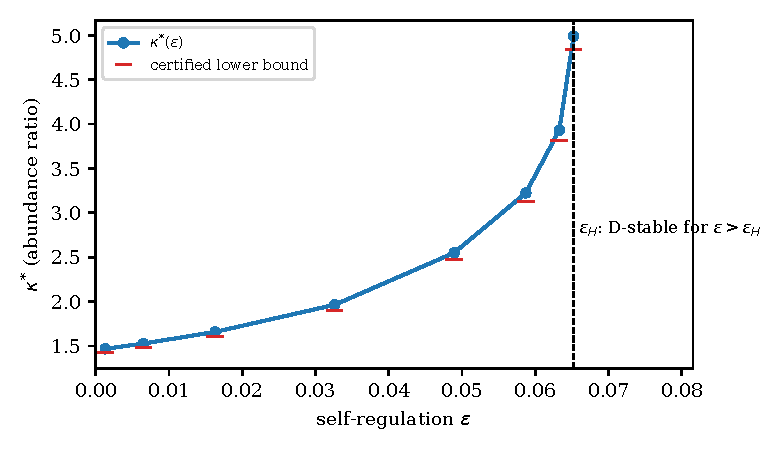
\includegraphics[width=0.72\linewidth]{figures/fig_w1.pdf}
\caption{Section~\ref{sec:w1}: $\ks(\varepsilon)$ on $(0,\varepsilon_H]$ with the certified lower bounds. D-stability holds
exactly for $\varepsilon>\varepsilon_H$; stability at equal abundances holds on the whole interval shown.}\label{fig:w1}
\end{figure}

\subsection{A published refinery-column gain matrix}\label{sec:w2}

Consider a stable, finite-dimensional, strictly proper plant $G(s)$ with integral loops $k_i/s$, negative feedback,
and the column sign normalization $G^{+}(0)=G(0)\diag(\operatorname{sign}g_{ii}(0))$. Campo and
Morari~\cite{CampoMorari1994} prove that the plant is decentralized integral controllable (DIC) if every principal
submatrix of $-G^{+}(0)$ is D-stable in our convention (Thm.~8), and that DIC requires every principal submatrix of
$-G^{+}(0)$ to be nonsingular and weakly D-stable, i.e.\ every scaling $DM$ with $D>0$ has its spectrum in the
closed left half-plane (Thm.~7); D-stability of $G(0)$ alone is not equivalent to
DIC~\cite[Ex.~3]{CampoMorari1994}. In the low-gain regime the slow closed-loop modes follow $\dot x=-G^{+}(0)Kx$
with $K$ the diagonal gain matrix, so $\ks(-G^{+}(0))$ is the least loop-gain ratio that destabilizes them.

We use the $4\times4$ steady-state gain matrix of an industrial naphtha column at the Al-Doura refinery, identified
by pulse tests~\cite[eq.~(27)]{MahmoodAlzobai2026}. Two caveats apply. Its input $X_f$ (feed composition) is a
disturbance rather than a manipulated variable, and the model has dead times, which lie outside the finite-dimensional
setting of~\cite{CampoMorari1994}. We therefore report total D-stability of $-G^{+}(0)$ for the published $4\times4$
matrix, and interpret it as DIC only for the $3\times3$ subsystem of manipulated inputs $(R,Q_R,F)$ paired with
$(X_D,X_B,B)$, and only for the delay-free model with the same steady-state gain. As a check we also treat the
sidestream column of Elaahi and Luyben~\cite{ElaahiLuyben1985}, as reprinted in~\cite[Ex.~3]{SkogestadMorari1992},
known not to be DIC for the diagonal pairing; the eigenvalues of $G^{+}(0)$ computed from the reprinted entries agree
with the values printed there. No verifiable $5\times5$ gain matrix of a real process was found.

\begin{table}[h]
\centering\small
\caption{Total D-stability of $-G^{+}(0)$ (diagonal pairing). $1\times1$, $2\times2$ (the $P_0^+$
test~\cite{JohnsonCR1974JRNBS}) and $3\times3$ (Cain~\cite{Cain1976}) principal submatrices are decided exactly. A
diagonal Lyapunov certificate for the whole matrix implies D-stability of every principal submatrix, because it
restricts to them; for the Al-Doura $4\times4$ matrix this implication and the certificate are checked in Lean.}\label{tab:w2}
\begin{tabular}{@{}L{0.25\linewidth}L{0.17\linewidth}L{0.2\linewidth}L{0.29\linewidth}@{}}
\toprule
Gain matrix & eigenvalues of $G^{+}(0)$ & principal submatrices of $-G^{+}(0)$ not D-stable & verdict \\
\midrule
Al-Doura naphtha column, $4\times4$~\cite{MahmoodAlzobai2026} & $1.25$, $1.61$, $17.86\pm3.45i$ & none & totally D-stable; diagonal Lyapunov certificate $P=\diag(2/5,2/5,81/10,4/5)$ (Lean); $\ks=\infty$ \\
same, manipulated inputs $(R,Q_R,F)$ only, $3\times3$ & $0.79$, $1.65$, $23.15$ & none & totally D-stable; diagonal Lyapunov certificate $P=\diag(7/10,4/5,9/5)$; $\ks=\infty$ \\
Elaahi--Luyben sidestream column, $4\times4$~\cite{ElaahiLuyben1985,SkogestadMorari1992} & $-9.69$, $4.74$, $6.05$, $19.88$ & \{1,3\}; \{1,4\}; \{2,4\}; \{3,4\}; \{1,2,3\}; \{1,2,4\}; \{1,3,4\}; \{2,3,4\}; \{1,2,3,4\} & not totally D-stable; every listed submatrix is not even Hurwitz, so $\ks=1$ for it \\
\bottomrule
\end{tabular}

\end{table}

\subsection{Known families as boundary types}\label{sec:w3}

Table~\ref{tab:families} places the benchmark families on the two sides of the dichotomy of
Theorem~\ref{thm:dichotomy}. Figure~\ref{fig:geography}, Table~\ref{tab:exponents} and
Figure~\ref{fig:divergence} describe the certified boundary atlas of Section~\ref{sec:validation}. There a bracket is
called a \emph{face birth} if its unstable endpoint has an exact face certificate (an exact Routh count $>0$ at a
scaling with one group of rates $10^k$ times the others), and an \emph{interior birth} otherwise; these are heuristic
proxies for escape and tangential boundary points, not certified classifications. Along interior-birth segments $\ks$
stays bounded ($p\approx0$ in Table~\ref{tab:exponents}). Along face-birth segments it diverges: 20 of the 21
segments give $p$ between $0.81$ and $1.07$, as Remark~\ref{rem:p1} predicts for one fast index (the same exponent is
observed for larger fast sets), and one random face-birth segment grows faster, by a factor of about $16$ per factor
$4$ in $\delta$ over most of its range ($p\approx2$; its fitted value $3.22$ is driven by the bound at the smallest
distance). Faster growth is expected when the crossing of the slow system is degenerate ($\alpha=0$ in
Remark~\ref{rem:p1}).

\begin{table}[h]
\centering\small
\caption{Boundary types of benchmark families.}\label{tab:families}
\begin{tabular}{@{}L{0.3\linewidth}L{0.2\linewidth}L{0.42\linewidth}@{}}
\toprule
Family & boundary type & evidence \\
\midrule
$B(h)$ window edges $h_\pm$ \cite{companion_attach} & escape & $h_\pm$ recovered exactly as roots of Cain's equality for a Schur complement; $\ks\sim\delta^{-1}$ (Table~\ref{tab:exponents}) \\
coNP gadgets (Pell cores with one attachment) \cite{companion_conp} & escape (heuristic) & exact face certificates at 40 of 40 certified births; $\ks$ grows like $\delta^{-1}$ (Table~\ref{tab:exponents}) \\
$B_3$ (Example~\ref{ex:b3}) & tangential & exact: unique contact, of rank one; $\ks=3$ \\
$D_0A_\varepsilon$, $\varepsilon=1/1000$ (Example~\ref{ex:tangential}) & tangential contact & exact contact of rank one; isolated (Jacobian rank 6) \\
community $S(J-\varepsilon I)$ at $\varepsilon_H$ (Section~\ref{sec:w1}) & tangential & $\ks\to5$ as $\varepsilon\uparrow\varepsilon_H$ \\
circulant $J-\varepsilon I$ (normal) & -- & D-stable iff Hurwitz; $P=I$ certifies for $\varepsilon>\varepsilon_H$ \\
\bottomrule
\end{tabular}

\end{table}

\begin{figure}[h]
\centering
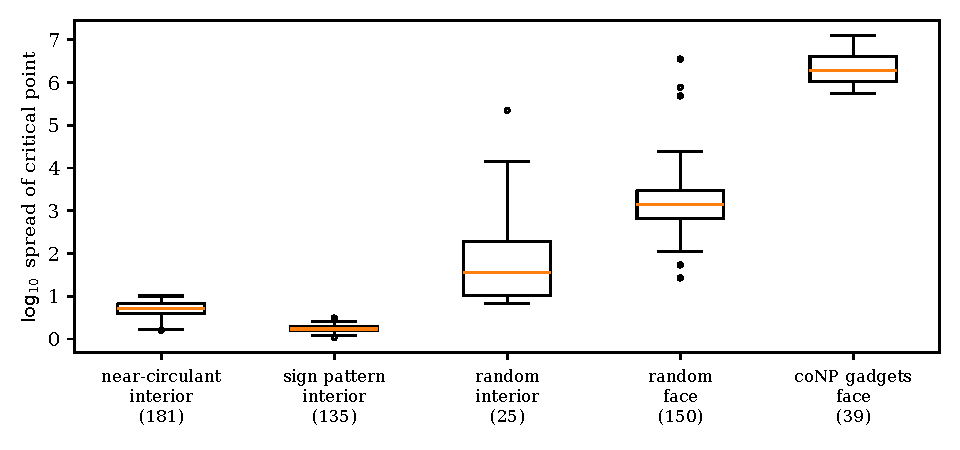
\includegraphics[width=0.9\linewidth]{figures/fig_geography.pdf}
\caption{Certified boundary atlas: spread of the $\psi$-minimal critical point at the unstable endpoint of a
certified bracket (an upper bound for $\ks$), by matrix class and birth type, for the 530 of the 538 brackets of
Section~\ref{sec:validation} whose critical point was recorded; counts in parentheses. The classes are defined in
Section~\ref{sec:validation}.}\label{fig:geography}
\end{figure}

\begin{table}[h]
\centering\small
\caption{Divergence of $\ks$ at distance $\delta$ from atlas boundary points, one row per birth type: exponent $p$ in
$\ks\asymp\delta^{-p}$, fitted per segment to the certified upper bounds (exact Routh certificates) at the four
smallest distances $\delta\in\{2^{-2},2^{-4},\dots,2^{-20}\}$ where a certificate exists; values of $\ks$ above about
$10^{7}$ could not be certified in double precision and are not used.}\label{tab:exponents}
\begin{tabular}{@{}lrrr@{}}
\toprule
Segments & count & median $p$ & range of $p$ \\
\midrule
face births, coNP gadgets & 10 & 0.99 & [0.81, 1.03] \\
face births, random & 11 & 1.00 & [0.83, 3.22] \\
interior births, near-circulant & 10 & 0.01 & [0.00, 0.01] \\
interior births, sign pattern & 10 & 0.02 & [0.02, 0.02] \\
$B(h)$ at $h_{-}$ (Example~\ref{ex:bh}) & 1 & 0.971 & -- \\
$B(h)$ at $h_{+}$ (Example~\ref{ex:bh}) & 1 & 0.995 & -- \\
\bottomrule
\end{tabular}

\end{table}

\begin{figure}[h]
\centering
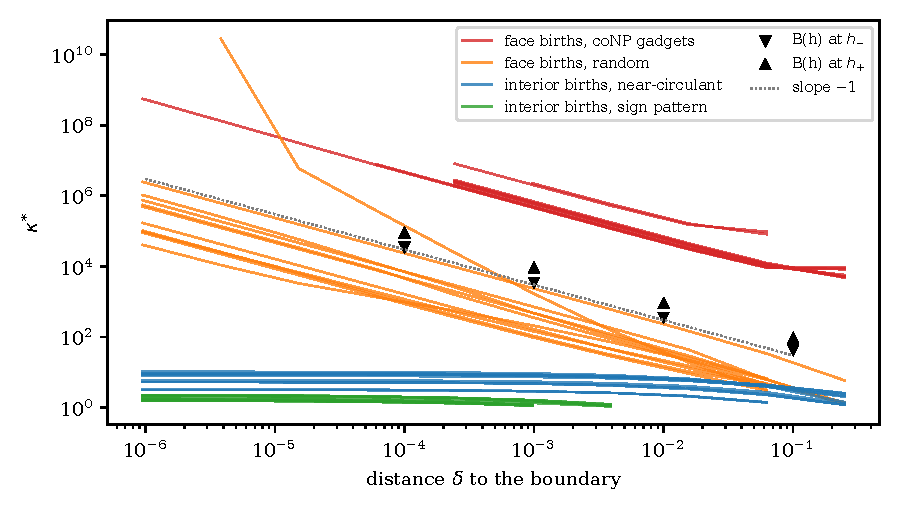
\includegraphics[width=0.8\linewidth]{figures/fig_divergence.pdf}
\caption{$\ks$ (certified upper bounds) versus the distance $\delta$ to the boundary on the atlas segments of
Table~\ref{tab:exponents}: along face-birth segments $\ks$ diverges, in all but one case like $\delta^{-1}$; along
interior-birth segments it stays bounded. Black markers: the $B(h)$ window edges of
Example~\ref{ex:bh}.}\label{fig:divergence}
\end{figure}

\subsection{Runtime}\label{sec:w4}

Table~\ref{tab:runtime} reports the wall-clock time of the complete $5\times5$ decision (compiled parameter homotopy
for (b), exact face checks, and an independent certificate) on 120 certified boundary instances of the atlas, on a
shared workstation. All 120 verdicts agree with the independent certification of the atlas; \WfourCerts.

\begin{table}[h]
\centering\small
\caption{Time per $5\times5$ decision (seconds).}\label{tab:runtime}
\begin{tabular}{@{}lrrr@{}}
\toprule
Instances & count & median & 95th percentile \\
\midrule
near-circulant, stable endpoint & 15 & 3.91 & 4.90 \\
near-circulant, unstable endpoint & 15 & 0.54 & 0.96 \\
sign pattern, stable endpoint & 15 & 3.60 & 4.72 \\
sign pattern, unstable endpoint & 15 & 0.84 & 1.00 \\
random, stable endpoint & 15 & 3.01 & 13.26 \\
random, unstable endpoint & 15 & 0.70 & 1.07 \\
coNP gadgets, stable endpoint & 15 & 2.76 & 3.18 \\
coNP gadgets, unstable endpoint & 15 & 0.63 & 2.21 \\
\midrule
all & 120 & 2.26 & 4.85 \\
\bottomrule
\end{tabular}

\end{table}

\section{Validation of the implementation}\label{sec:validation}

\paragraph{Test matrices.} The calibration suite consists of 27 matrices of order $5$ with independently known verdicts: $3\times3$ matrices on or near the boundary of Cain's criterion, embedded block-diagonally, weakly coupled or bordered; the family $B(h)$ of Example~\ref{ex:bh} at $h=4,5,6$, bordered; vertex and off-vertex matrices of the coNP-hardness gadgets of~\cite{companion_conp}; perturbations of the circulant core $J$ of Section~\ref{sec:w1}, including Example~\ref{ex:tangential}; matrices with negative definite symmetric part; matrices with a non-D-stable $3\times3$ principal submatrix; and a family with symmetric principal minors. The boundary atlas uses segments $t\mapsto(1-t)A_s+tA_u$ from an exactly certified D-stable $A_s$ to an exactly certified non-D-stable $A_u$ in four classes: \emph{random} ($A_s=-(MM^{\mathsf T}+I)+W-W^{\mathsf T}$ with small random integer matrices $M,W$, which is diagonally stable, and a random $A_u$); \emph{near-circulant} ($D_0(J_q-\frac1{100}I)$ with a random positive diagonal $D_0$ and a circulant $J_q$ moved from a D-stable to an unstable parameter); \emph{sign pattern} (negative diagonal, $a_{i,i+1}>0$, $a_{i+2,i}<0$ cyclically, random magnitudes); and \emph{coNP gadgets} (Pell cores with one attachment~\cite{companion_conp}). A \emph{certified bracket} is a subsegment of relative width at most $10^{-3}$ whose endpoints are certified D-stable and non-D-stable independently of the criterion.

\paragraph{Calibration.} All 27 calibration matrices are decided correctly, with 27 certified verdicts and 0 disagreements.

\paragraph{Boundary atlas.} In a first design (70 segments, 69 certified brackets), bisection used a multistart growth-rate sampler; the criterion found real positive critical points at 23 points that the sampler had labelled stable, and an exact Routh count confirmed strict D-instability at every one of them. In a second design (473 segments, 472 certified brackets, 3 of them certified after the run by a rigorous exclusion with a larger budget) bisection used the criterion's own verdict (compiled parameter homotopy), and every bracket endpoint was certified independently, in the direction the criterion predicted. Of the 541 certified brackets, the stable endpoints carry 363 exact diagonal Lyapunov certificates and 178 rigorous exclusions (Appendix~\ref{app:exclusion}); the unstable endpoints carry 536 exact Routh counts, and 5 are not Hurwitz. With the 23 corrected points this gives 1105 certified instances concentrated at the boundary, with no unresolved disagreement.

\paragraph{One genuine disagreement.} In one further bracket of the second design the implementation reported no critical point at an endpoint that is in fact strictly D-unstable (exact Routh certificate at $d=(1,1,1,10^8,6\cdot10^7)$): a Schur-complement face of a coNP-gadget matrix places the critical point at spread $\gtrsim10^8$, beyond double-precision path tracking. The independent certification refused the bracket, so it is not among the certified brackets. The implementation now runs an exact face test before any stability certificate: for each index set $F$ it evaluates an exact Routh count at $d_F=10^k$ ($k\le12$), which can only certify instability. The defect is in the floating-point implementation, not in Theorem~\ref{thm:explicit}, whose critical point exists by Theorem~\ref{thm:coverage}.

\paragraph{Invariance and $n=3$.} The Lagrange verdict is the same for three exhaustions (log barrier with unit and random weights, reciprocal) on 23/24 Hurwitz calibration matrices; the exception is a path-tracking miss of the reciprocal system at spread $5\cdot10^4$; direct constrained minimization of the reciprocal exhaustion on $C_A$ recovers the missed critical point. The criterion reproduces Cain's exact $3\times3$ criterion on 60/60 random matrices embedded as $\diag(A_3,-1,-2)$.

\paragraph{Births.} Of the 538 distinct brackets certified during the runs, 192 have an exact face certificate at the unstable endpoint (an exact Routh count $>0$ at $d_F=10^k$, $k\le12$, for some index set $F$) and 346 do not; we call them face and interior births. Face births occur in the random (152 of 177) and coNP-gadget (40 of 40) classes; all near-circulant (181) and sign-pattern (140) births are interior births.

\paragraph{Census.} On the 532 certified brackets of the validation runs (pilot runs excluded) the compiled homotopy found a real positive critical point at every one of the 527 Hurwitz unstable endpoints (the other unstable endpoints are not Hurwitz) and none at any of the 532 stable endpoints. On the 24 Hurwitz calibration matrices it found one for every non-D-stable matrix except Example~\ref{ex:tangential}, which branch (c) decides, and for no D-stable matrix.


\section{Limitations and open problems}\label{sec:limits}

\begin{itemize}
\item \emph{Decision procedure.} Lean verifies the criteria as equivalences. The finite procedure also uses
Proposition~\ref{prop:fin} (sketch) and Lemma~\ref{lem:termination} (conventional) and has not been executed at $n=5$;
our verdicts come from floating-point homotopy together with independent exact or rigorous certificates, and branch (c)
is used only through exact contacts. Double-precision path tracking loses critical points of spread $\gtrsim10^8$, which
occur near faces of the orthant; the implementation compensates with exact face checks. An exact run at $n=5$
would need a zero-dimensional solver (Gr\"obner basis and real-root isolation) for (b), which has at most $1200$
isolated solutions for generic weights, and the recursion of Lemma~\ref{lem:termination} for (c), whose radicals,
singular loci and saturations are likely the costlier part; we have not attempted it.
\item \emph{Formalization.} Proposition~\ref{prop:fin}, Proposition~\ref{prop:bezout} as a bound on solutions,
Lemma~\ref{lem:termination} and the decision procedure are not formalized: Mathlib lacks algebraic generic
smoothness, multihomogeneous B\'ezout bounds, dimension theory of singular loci and real root isolation.
\item \emph{Divergence exponent.} Remark~\ref{rem:p1} is a sketch without a proved lower bound.
\item \emph{Finiteness of tangency sets.} We do not know whether the real tangency set of a Hurwitz matrix with coprime
$\Pre,\Pim$ is finite; Lemma~\ref{lem:termination} makes this an efficiency question.
\item \emph{Complexity of bounded-ratio stability.} Is $\kappa$-stability coNP-hard in $n$ for fixed $\kappa$?
\item \emph{Deficiency.} Does a $5\times5$ D-stable matrix exist all of whose proper principal submatrices of order at
least $2$ fail to be D-stable?
\item \emph{Nonlinear onset.} The results concern linear stability of equilibria.
\item \emph{Literature.} We were unable to consult the full texts of Burlakova~\cite{Burlakova2009} and
Pavani~\cite{Pavani2018,Pavani2019}.
\end{itemize}

\section{Formal verification}\label{sec:lean}

The development \path{proofs/DStability5x5/} has the root module \path{Paper.lean}, which builds on a pinned Mathlib
with Lean v4.30.0. The root and its import closure comprise 47 local modules: 14 in \path{proofs/DStability5x5/},
23 in \path{proofs/DUnstableCores/}, one in \path{proofs/DStabilityCharacterization/} and 9 in three further
directories. The basic notions (\texttt{DStable}, \texttt{HurwitzStable}, \texttt{HasEigenpair}, right scaling) come
from \path{proofs/DUnstableCores/DScaling.lean} and the continuation lemma from
\path{proofs/DStabilityCharacterization/SpectralContinuation.lean}; several modules of the closure are unrelated to
this paper and are compiled only because of imports. Every module compiles with warnings treated as errors and without
\texttt{sorry}; the exported declarations use only the axioms \texttt{propext}, \texttt{Classical.choice} and
\texttt{Quot.sound}. D-stability is formalized literally: for every $d>0$, every eigenpair of $A\diag d$ over $\C$ has
negative real part. Statements marked conventional, sketch, exact or numerical are not formalized.

\begin{table}[h]
\centering\small
\caption{Lean correspondence (namespace \texttt{DStability5x5}).}\label{tab:lean}
\begin{tabular}{@{}L{0.25\linewidth}L{0.5\linewidth}L{0.19\linewidth}@{}}
\toprule
Statement & Declaration & Module \\
\midrule
Lemma~\ref{lem:expansion} & \lean{contactDet_expansion}, \lean{pminor_eq_minorR} & ContactExpansion, PrincipalMinor \\
Lemma~\ref{lem:johnson} & \lean{dStable_iff_no_contact} & Cone \\
Theorem~\ref{thm:coverage} & \lean{dStable_iff_morseFor}, \lean{dStable_iff_morse_logBarrier} & ProperExhaustion \\
Theorem~\ref{thm:explicit} & \lean{dStable_iff_explicit} & ExplicitCriterion \\
Corollary~\ref{cor:branches} & \lean{dStable_iff_lagrange_tangency} & FiveByFive \\
Theorem~\ref{thm:five} & \lean{dStable_iff_five} & FiveByFive \\
Lemma~\ref{lem:singular} & \lean{not_surjective_iff_tangency}, \lean{regular_iff_rank} & Boundary, Robustness \\
Theorem~\ref{thm:robust} & \lean{exists_contact_near_of_regular}, \lean{not_dStable_near_of_regular} & Robustness \\
Corollary~\ref{cor:closure} & \lean{not_regular_of_mem_closure}, \lean{isOpen_hurwitz_regularContact}, \lean{hurwitz_regularContact_open_not_dStable} & Robustness \\
Theorem~\ref{thm:dichotomy} & \lean{closure_dichotomy} & Boundary \\
Theorem~\ref{thm:cone} & \lean{kStable_iff_no_cone_contact}, \lean{kStable_iff_no_boxFaceCritical}, \lean{dStable_iff_forall_kStable}, \lean{kStable_mono} & Cone \\
Proposition~\ref{prop:kappa}(a) & \lean{exists_least_unstable_ratio} & KappaStar \\
Theorem~\ref{thm:separation} & \lean{eventually_kStable_of_no_contact}, \lean{contact_of_tendsto_not_kStable} & Separation \\
Table~\ref{tab:w2} & \lean{dStable_of_diagLyapunov}, \lean{alDoura_dStable} & Lyapunov, AlDoura \\
\bottomrule
\end{tabular}
\end{table}

\paragraph{Replay.} The script \path{check_paper.py} recomputes every number printed in this paper from exact
arithmetic or from the stored evidence (\CheckCount); the ancillary directory contains the Lean modules, path-free
verification receipts with source hashes, and a command-line implementation of the decision procedure with its
certificates.

\appendix
\section{Rigorous exclusion of contacts}\label{app:exclusion}

For each of the $2^n$ charts $d_i=t_i$ or $d_i=1/t_i$ with $t\in[0,1]^n$, multiplying $f_A$ by the product of the
$t_i$ of the inverted coordinates gives a multiaffine polynomial $\tilde f$ in $t$ whose values at the corners of
$[0,1]^n$ are monomials of $f_A$ (for instance $i^n$ and $\det(-A)$); every positive $d$, including the limits
$d_i\to0$ and $d_i\to\infty$, is covered. By the multiaffine mapping theorem, $\tilde f(\text{box})$ lies in the convex
hull of the values of $\tilde f$ at the $2^n$ vertices of the box. A box is discarded if a unit vector $w$ satisfies
$\langle w,\tilde f(v)\rangle>\sqrt2\,\mathrm{err}(v)$ at every vertex $v$, where $\mathrm{err}(v)=64u\sum_S|c_S|t^S$
bounds the floating-point error of evaluating $\tilde f(v)$ with unit roundoff $u$ (the coefficients $c_S$ are the
principal minors, rounded once). Otherwise the box is bisected along its longest side. For a $\kappa$-stability
certificate, boxes that contain no point of $\Kk$ (some ratio $d_i/d_j$ exceeds $\kappa$ on the whole box) are pruned.
If every box is discarded and $A$ is Hurwitz (exact Routh test), $A$ is $\kappa$-stable (or D-stable, without pruning)
by Theorem~\ref{thm:cone}(a). The implementation is in the ancillary files.

\bibliographystyle{plain}
\bibliography{refs}
\end{document}
